\documentclass[10pt]{article}
\usepackage[a4paper,margin=1in]{geometry}
\usepackage{graphicx}
\usepackage{titlesec}
\usepackage{parskip}
\usepackage{enumitem}
\usepackage{multicol}
\usepackage{float}
\usepackage{booktabs}
\usepackage[most]{tcolorbox}
\usepackage{caption}

\titleformat{\section}{\normalfont\Large\bfseries}{}{0pt}{}
\titleformat{\subsection}{\normalfont\large\bfseries}{}{0pt}{}

\setlength{\columnsep}{1cm} % space between the columns
\setlength{\columnseprule}{0.4pt} % thickness of the vertical dividing line

\tcbset{
	colback=blue!5,    % light grey background
	colframe=black,     % border color
	boxrule=0.5pt,      % border thickness
	arc=1mm,            % rounded corners
	left=6pt, right=6pt, top=6pt, bottom=6pt, % Padding
}

\captionsetup[figure]{justification=centering}

\begin{document}
	
	\begin{center}
		\LARGE\textbf{Policy Brief: Is Peterborough More Divided by Ethnicity or Occupational Social Class?}
	\end{center}
	
	\begin{multicols}{2}
	
	\section*{Executive Summary}
	
	\begin{tcolorbox}
	\begin{itemize} [left=0.3em, labelsep=0.5em, labelwidth=0.6em, itemsep=0pt, topsep=0pt]
		\item Peterborough shows greater division by \textbf{ethnicity} (\textit{dissimilarity index: 0.379}) than by \textbf{occupational class} (\textit{0.313}).
		\item \textbf{Ethnic minorities} are concentrated in central areas, while \textbf{White residents} dominate peripheral zones.
		\item Occupational groups (NS-SEC 1-2 vs 5-7) also show spatial clustering, but with \textbf{greater overlap} between areas.
		\item Spatial analysis using \textbf{Getis-Ord Gi*} reveals \textbf{sharper ethnic hot/cold spots} than those for occupational groups.
		\item \textbf{Policy solutions} should prioritise place-based interventions that encourage ethnic mixing in housing, schools, and shared spaces, while also addressing underlying economic inequality.
	\end{itemize}
	\end{tcolorbox}
	
	\vspace{0em}

	\section*{Background and Context}
	\indent The 2016 \textit{Casey Review} warned of the risks posed by fragmented communities in the UK, particularly in areas where ethnic and religious groups rarely mix. It highlighted how such divisions can entrench disadvantage and erode social trust. In response, the UK Government introduced the \textit{Integrated Communities Strategy} Green Paper (2018) and Action Plan (2019), promoting mixed communities as a route to cohesion and prosperity. Drawing on contact theory, the Strategy argued that increased social mixing helps reduce prejudice and build stronger local ties. While socio-economic divisions were acknowledged, the primary focus remained on ethnic and religious integration. Peterborough was one of five areas chosen to pilot these efforts.
	
	\vspace{0em}
		
	\section*{Data and Methods}
	\indent This brief draws on 2021 Census Output Area (OA) data to examine spatial divisions in Peterborough by occupational class and ethnicity. Occupational groups were classified using the National Statistics Socio-Economic Classification (NS-SEC), comparing NS-SEC 1-2 (managerial/professional occupations) with NS-SEC 5-7 (routine/manual jobs). Ethnicity was simplified into a binary comparison between White populations (White British and Other White) and All Minority groups. Statistical and spatial techniques were used to analyse how these groups are distributed across Peterborough’s OAs. Boxplots were used to explore the variation in group distributions across OAs. Choropleth maps visualised group concentrations, while Getis-Ord Gi* statistics identified significant spatial clustering. An index of dissimilarity was calculated to quantify segregation, with values ranging from 0 (complete integration) to 1 (complete separation). 
	
	\vspace{-1em}
	
	\section*{Key Findings}
	
	\begin{figure}[H]
		\centering
		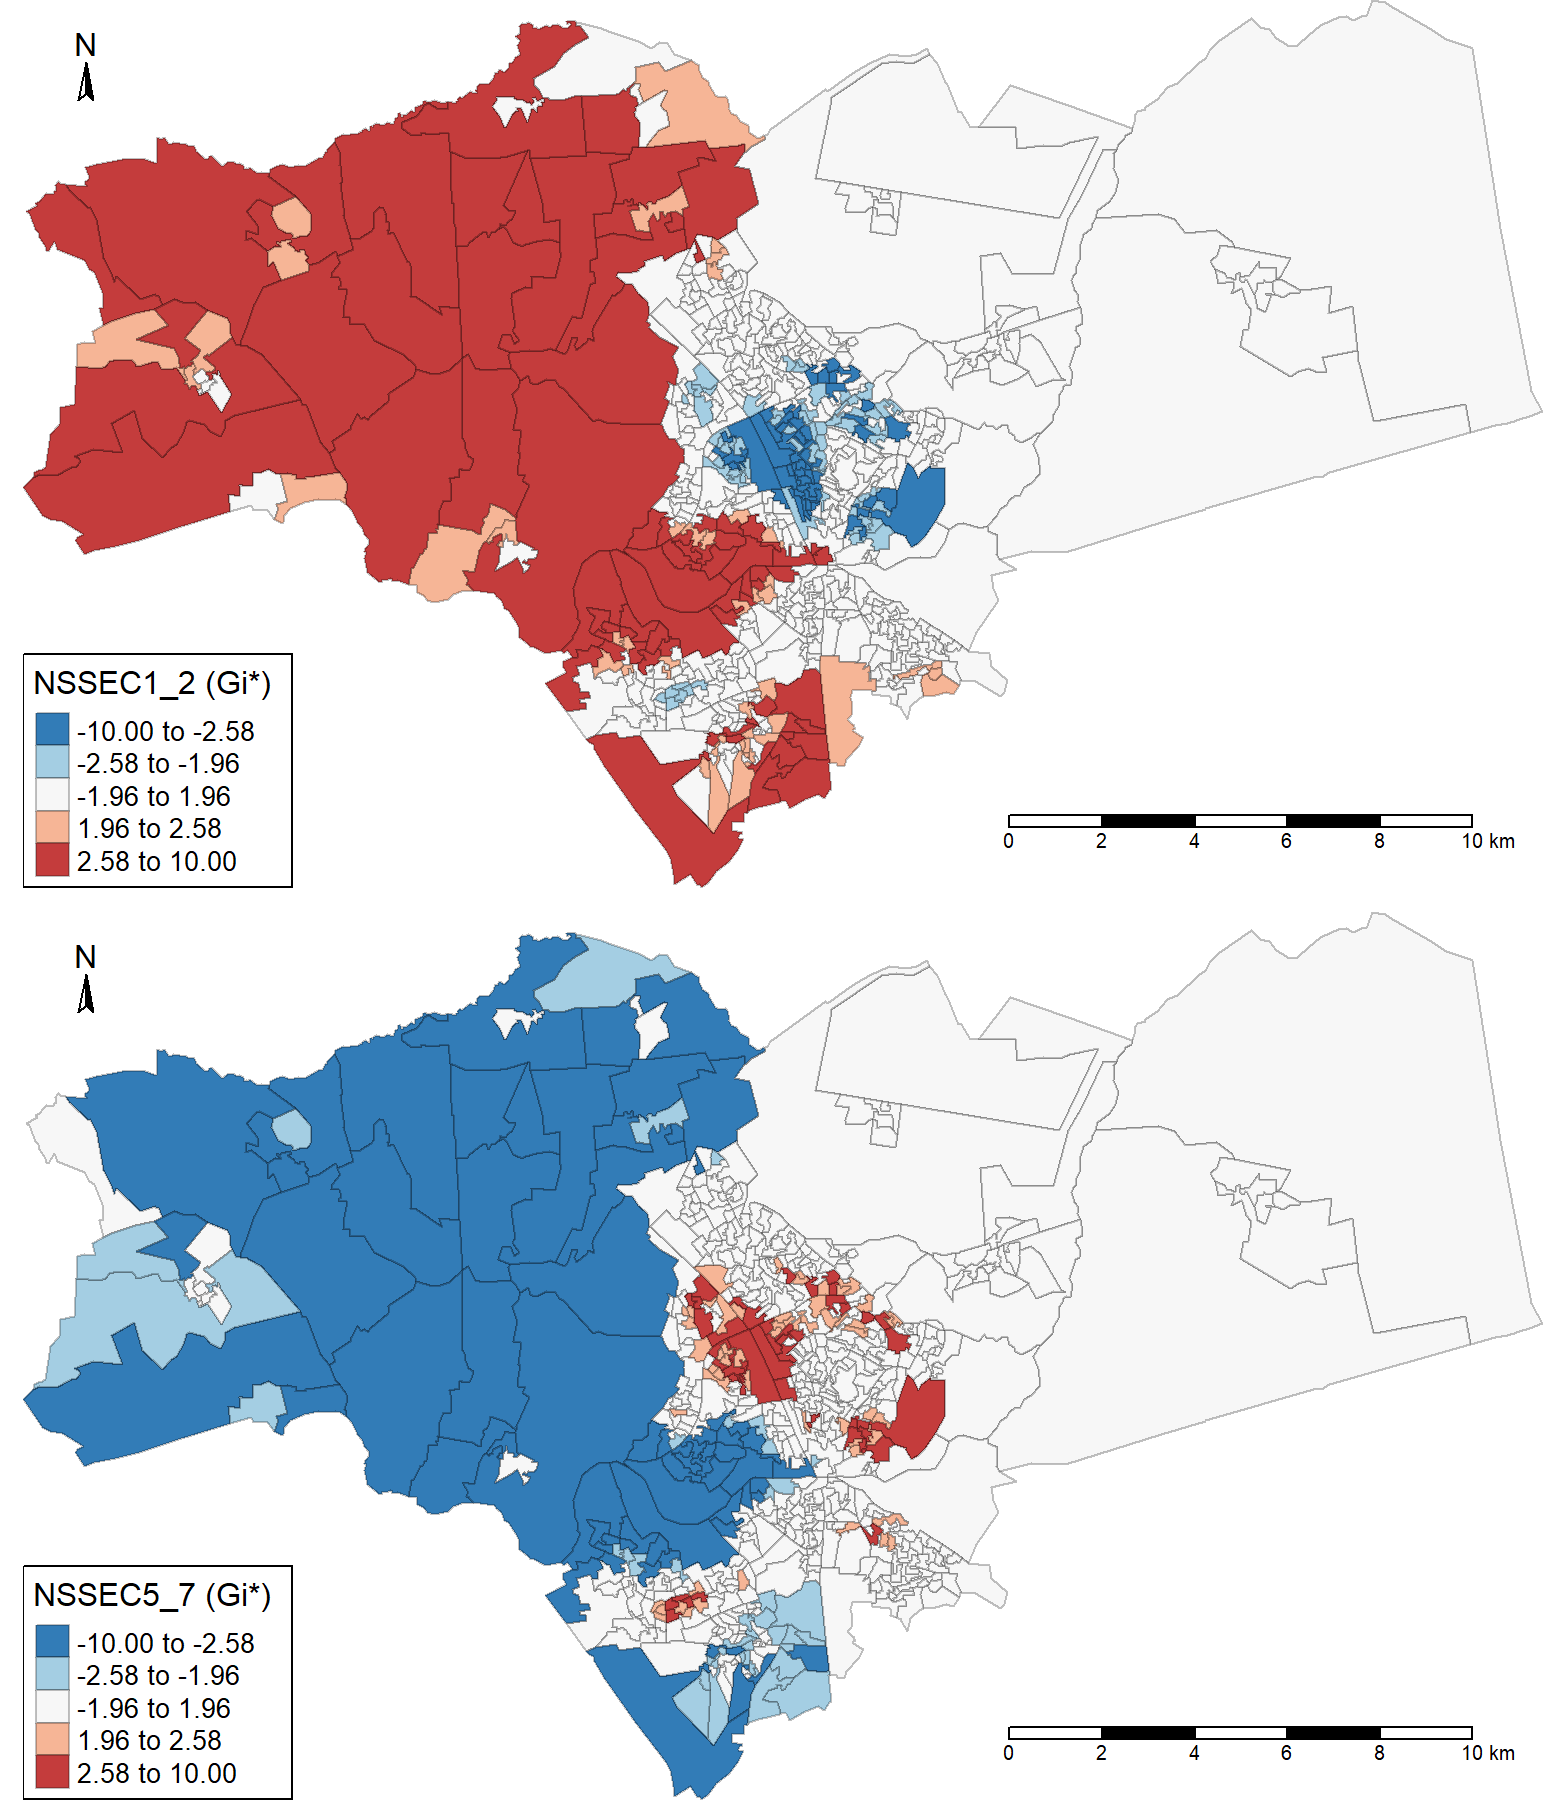
\includegraphics[width=0.8\linewidth]{occupation_gi.png}
		\caption{Hotspot and Coldspot Analysis for Occupational Groups (Gi*)}
		\label{fig:occupation_gi}
	\end{figure}

	\begin{figure}[H]
		\centering
		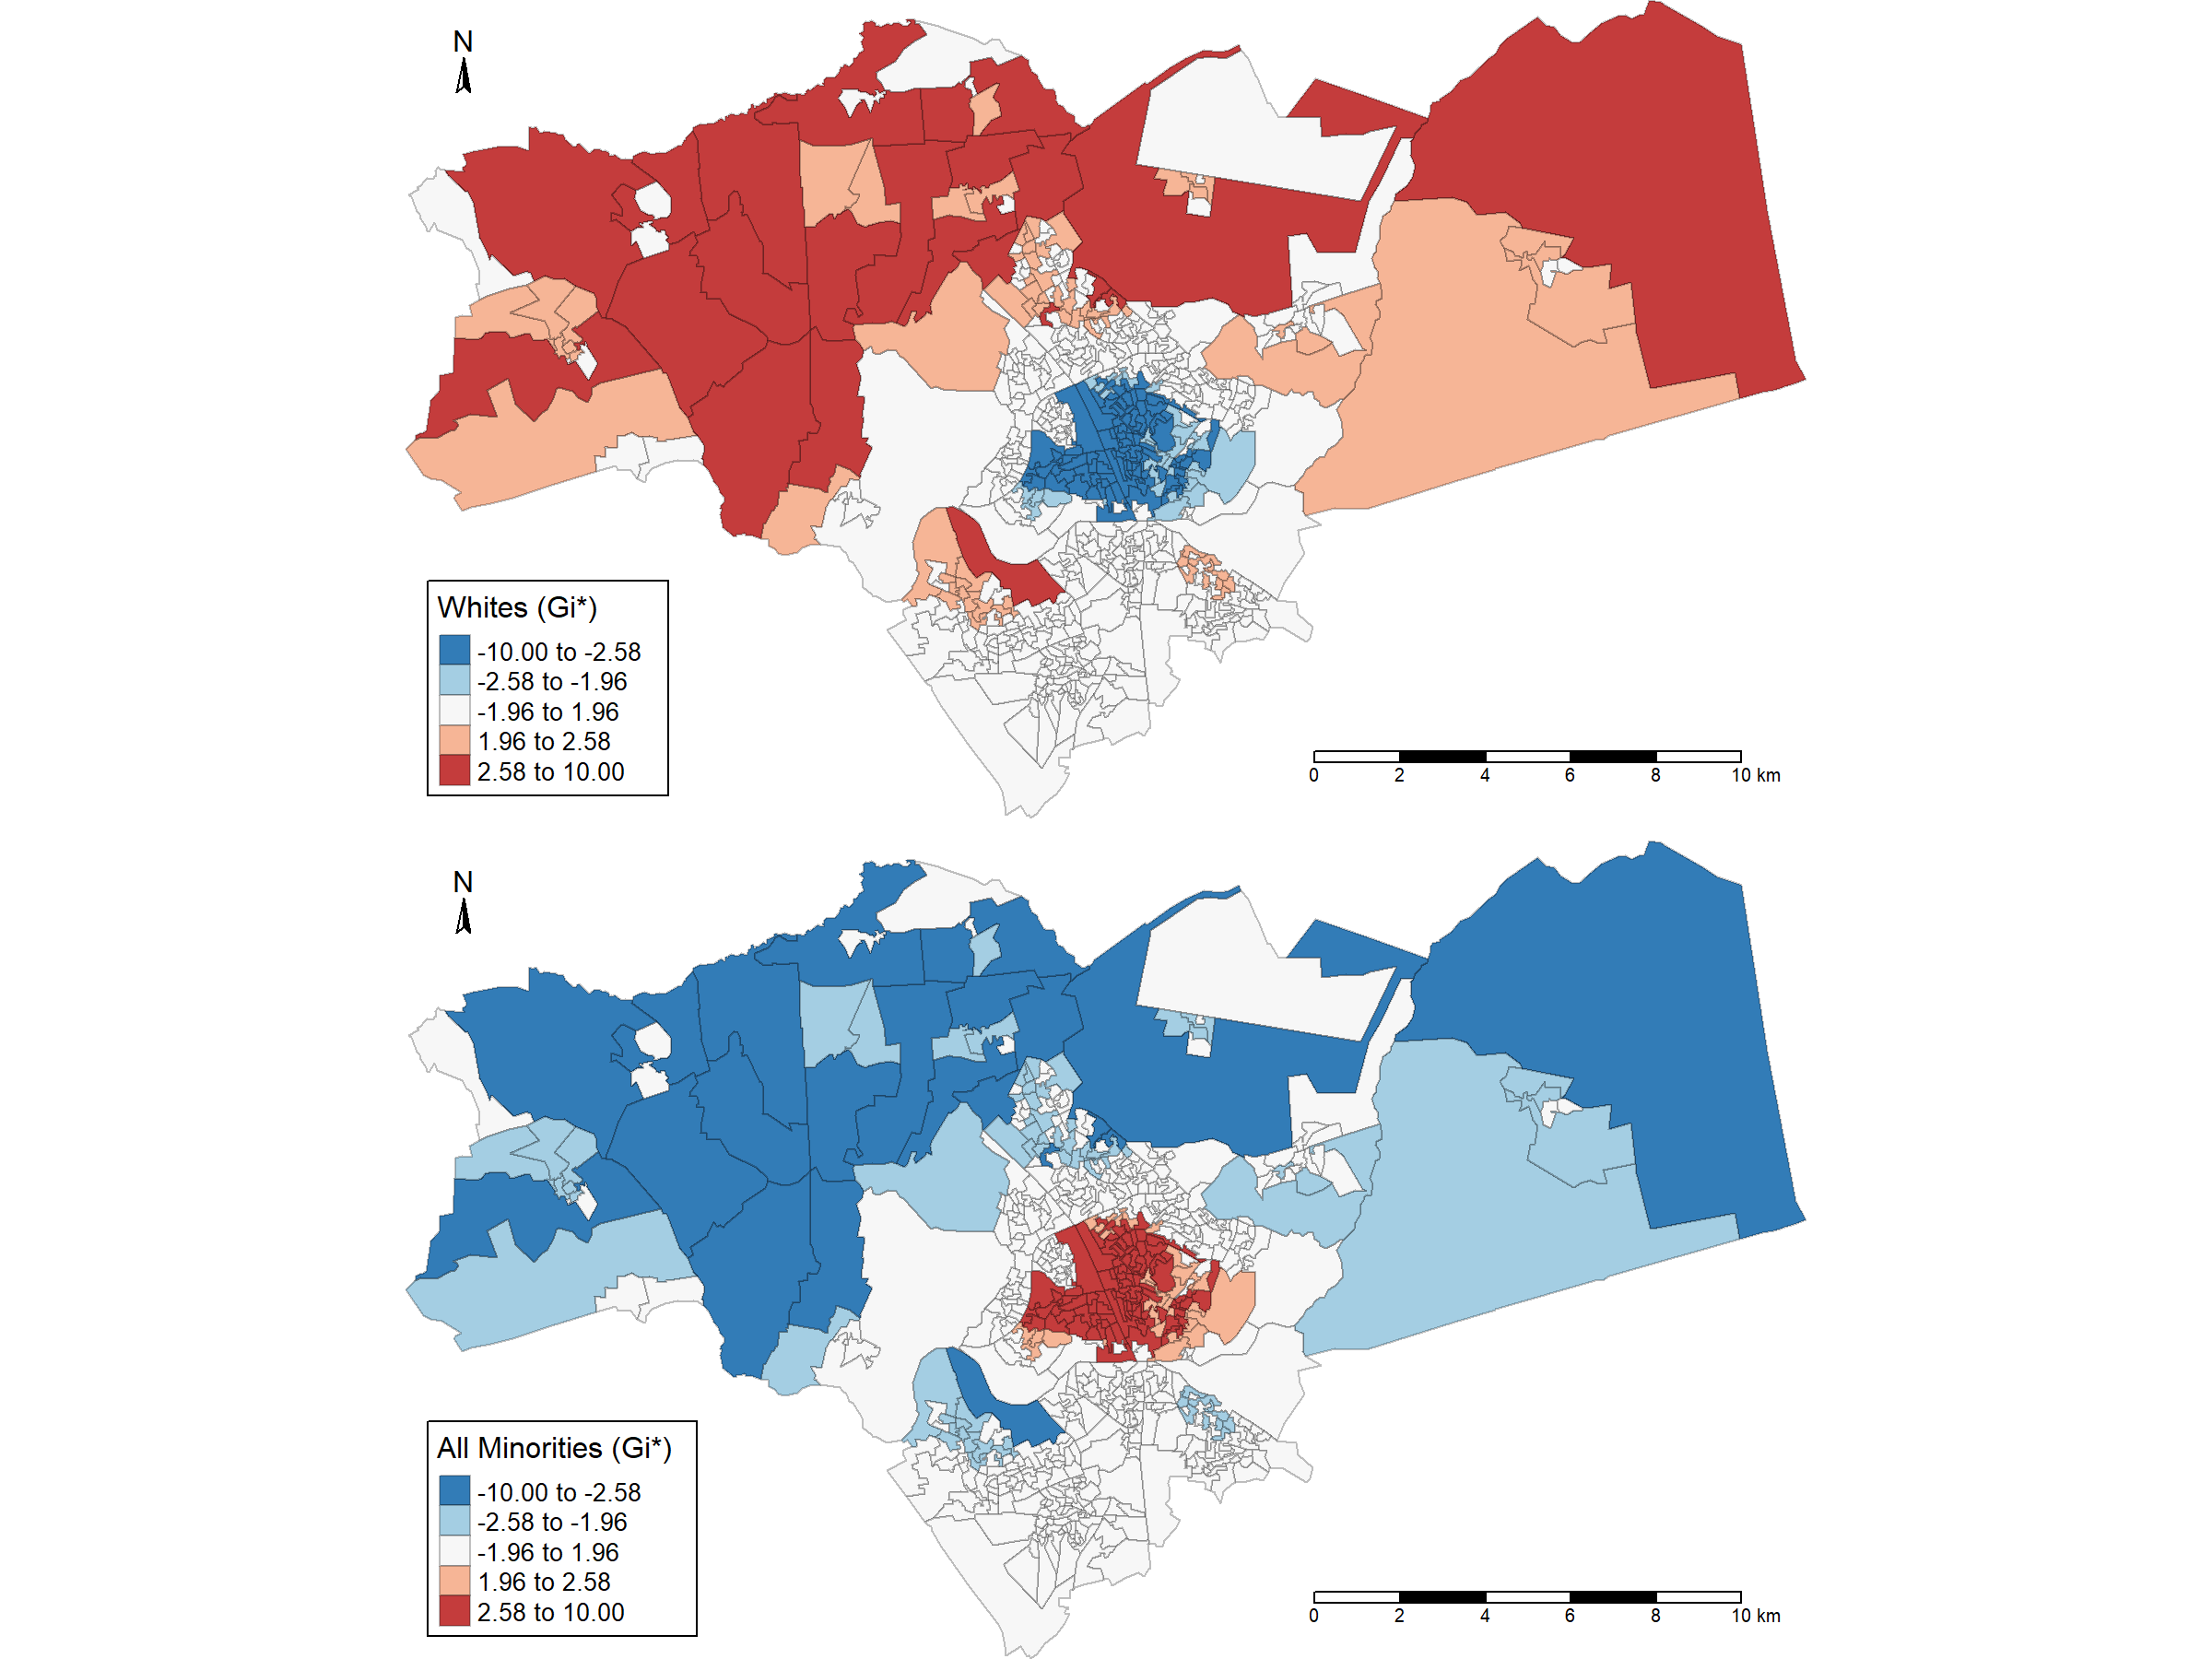
\includegraphics[width=0.8\linewidth]{ethnicity_gi.png}
		\caption{Hotspot and Coldspot Analysis for Ethnic Groups (Gi*)}
		\label{fig:ethnicity_gi}
	\end{figure}
	
	\begin{table}[H]
		\centering
		\caption{Index of Dissimilarity in Peterborough}
		\label{tab:dissimilarity}
		\begin{tabular}{lcc}
			\toprule
			City & ID\_Occupation & ID\_Ethnicity \\
			\midrule
			Peterborough & 0.313 & 0.379 \\
			\bottomrule
		\end{tabular}
	\end{table}

	\subsection*{Occupational Class Division}
	\indent Occupational data show that semi-routine and manual occupations (NS-SEC 5-7) make up an average of 36.3\% of Peterborough's OA populations, compared to 27.8\% for managerial and professional roles (NS-SEC 1-2). The wider distribution of NS-SEC 1-2 suggests some OAs are dominated by professionals, while others have minimal representation. Thematic maps and hotspot analysis indicate that professional roles are more common in suburban areas, while manual occupations cluster in the central and eastern parts of the city. The dissimilarity index for occupational groups is 0.313, reflecting a moderate level of spatial separation.
	
	\subsection*{Ethnic Division}
	\indent Ethnic segregation in Peterborough is more pronounced than occupational segregation. White British residents average 62.1\% of OA populations but ranges from just 3.7\% to 97.3\%, revealing sharp variation. Thematic maps clearly show that the outer zones of Peterborough are overwhelmingly White, while central areas are home to most minority populations. Hotspot analysis further support this, showing strong clustering of minority groups in the city centre. The dissimilarity index for ethnicity is 0.379, indicating greater spatial separation than for occupational class.
	
	\vspace{-1em}
	
	\section*{Policy Implications}
	\indent While contact theory (Allport, 1954) suggests that intergroup interactions can reduce prejudice, the spatial patterns in Peterborough imply limited opportunities for such contact, particularly in areas of high ethnic concentration. Although socio-economic inequality plays a role, the evidence points to ethnic residential segregation as a stronger driver of spatial division. This supports the concerns raised in the \textit{Casey Review} and underscores the need for integration policies that prioritise ethnic mixing while also addressing underlying economic disparities. We should also consider the role of intersectionality, as ethnic minorities are disproportionately represented in NS-SEC 5-7 occupations, reinforcing spatial inequalities.	
	
	\vspace{-1em}
		
	\section*{Recommendations}
	\indent To support greater integration in Peterborough, the City Council should prioritise locally targeted interventions that reflect the city's spatial dynamics. Housing policy can play a key role by promoting mixed-tenure and affordable developments in areas dominated by a single ethnic group, especially within new growth or in regeneration zones. Educational initiatives, such as encouraging diverse school intakes and joint extracurricular programmes, can help foster early social mixing. Shared community infrastructure is also vital: investing in inclusive public spaces, multicultural centres, and city-wide events can help bridge divides. Finally, the Council should continue building on its Integration Area status by using spatial data to monitor progress and collaborating with local partners to ensure that actions remain relevant and responsive to community needs.
	
	\vspace{-1em}
	
	\section*{Limitations}
	\indent This analysis simplifies complex realities by grouping ethnicity into "White" versus "All Minorities" and occupation into NS-SEC 1-2 versus 5-7. While this enables the identification of broad spatial patterns, it overlooks important variation within minority groups and among intermediate occupational classes such as NS-SEC 3-4. The cross-sectional nature of the study, relying solely on 2021 Census data, also limits its ability to capture how segregation may evolve in response to future migration, policy interventions, or socio-economic change.
	
	\indent There are also spatial and methodological limitations. Although Output Areas provide relatively fine-grained data, the results remain subject to the Modifiable Areal Unit Problem (MAUP), meaning observed patterns might vary at different geographic scales. Occupational data exclude economically inactive populations, and the Gi* hotspot analysis is sensitive to how spatial relationships are defined. Finally, the study relies exclusively on quantitative methods, omitting qualitative perspectives that are essential to understanding how spatial division is experienced at the community level.
	
	\vspace{-1em}
	
	\section*{Conclusion}
	\indent Ethnicity remains the stronger axis of spatial division in Peterborough than occupational class. While both forms of segregation exist, ethnic separation is more pronounced and geographically entrenched. Integration policy must reflect this by prioritising efforts to reduce ethnic residential segregation, while also addressing economic disadvantages to avoid reinforcing social exclusion. A dual focus on ethnicity and class will be key to building a more integrated, cohesive, and equitable Peterborough.
	
	\end{multicols}
\end{document}
